%%%%%%%%%%%%%%%%%%%%%%%%%%%%%%%%%%%%%%%%%%%%%%%%%%%%%%%%%%%%%%%%%%%%%%
% Overleaf (WriteLaTeX) Example: Molecular Chemistry Presentation
%
% Source: http://www.overleaf.com
%
% In these slides we show how Overleaf can be used with standard 
% chemistry packages to easily create professional presentations.
% 
% Feel free to distribute this example, but please keep the referral
% to overleaf.com
% 
%%%%%%%%%%%%%%%%%%%%%%%%%%%%%%%%%%%%%%%%%%%%%%%%%%%%%%%%%%%%%%%%%%%%%%

\documentclass{beamer}

\mode<presentation>
{
  \usetheme{Madrid}       % or try default, Darmstadt, Warsaw, ...
  \usecolortheme{default} % or try albatross, beaver, crane, ...
  \usefonttheme{default}    % or try default, structurebold, ...
  \setbeamertemplate{navigation symbols}{}
  \setbeamertemplate{caption}[numbered]
} 

\usepackage[english]{babel}
\usepackage[utf8x]{inputenc}
\usepackage{chemfig}
\usepackage[version=3]{mhchem}

\usepackage{hyperref}
  \hypersetup{colorlinks=true}
  \hypersetup{urlcolor=blue}
  \hypersetup{linkcolor = .}
\usepackage{xcolor}
\usepackage{siunitx}
  \sisetup{separate-uncertainty = true}
\usepackage{physics}
\usepackage[font=small,labelfont=bf]{caption}
\usepackage{subcaption}
\usepackage[en-GB]{datetime2}
\usepackage{feynmp}
\DeclareGraphicsRule{*}{mps}{*}{}

\usepackage{scalerel}
\newcommand{\mylbrace}[2]{\vspace{#2pt}\hspace{6pt}\scaleleftright[\dimexpr5pt+#1\dimexpr0.06pt]{\lbrace}{\rule[\dimexpr2pt-#1\dimexpr0.5pt]{-4pt}{#1pt}}{.}}
\newcommand{\myrbrace}[2]{\vspace{#2pt}\scaleleftright[\dimexpr5pt+#1\dimexpr0.06pt]{.}{\rule[\dimexpr2pt-#1\dimexpr0.5pt]{-4pt}{#1pt}}{\rbrace}\hspace{6pt}}

% Here's where the presentation starts, with the info for the title slide
\title[BESIII Oxford]{BESIII Oxford Group Meeting}
\author{Martin Tat}
\institute{Oxford LHCb}
\date{25th February 2021}

\titlegraphic{
\includegraphics[width = 5cm, height = 3.8cm]{lhcb.jpg}\hspace{1cm}~%
              
\includegraphics[width = 5cm, height = 3.8cm]{bes3.png}}

\begin{document}

\begin{frame}
  \titlepage
\end{frame}

% These three lines create an automatically generated table of contents.
%\begin{frame}{Outline}
%  \tableofcontents
%\end{frame}

\section{Introduction}
\begin{frame}{Introduction}
  \begin{itemize}
    \item{Previously: Single tagged $D\to K^+K^-\pi^+\pi^-$ events}
    \item{Current progress: Double tagged $D\to K^+K^-\pi^+\pi^-$ events}
    \item{Tag modes:}
    \begin{itemize}
      \item{$K\pi$, $KK$, $K_S\pi^0$, $K\pi\pi^0$}
    \end{itemize}
    \item{Ran over $50\%$ of the $2010$ MC $D^0\bar{D}^0$ sample}
  \end{itemize}
\end{frame}

\section{Double tags}
\begin{frame}{$K\pi$ tag}
  \begin{figure}
    \centering
    \begin{subfigure}{0.5\textwidth}
      \centering
      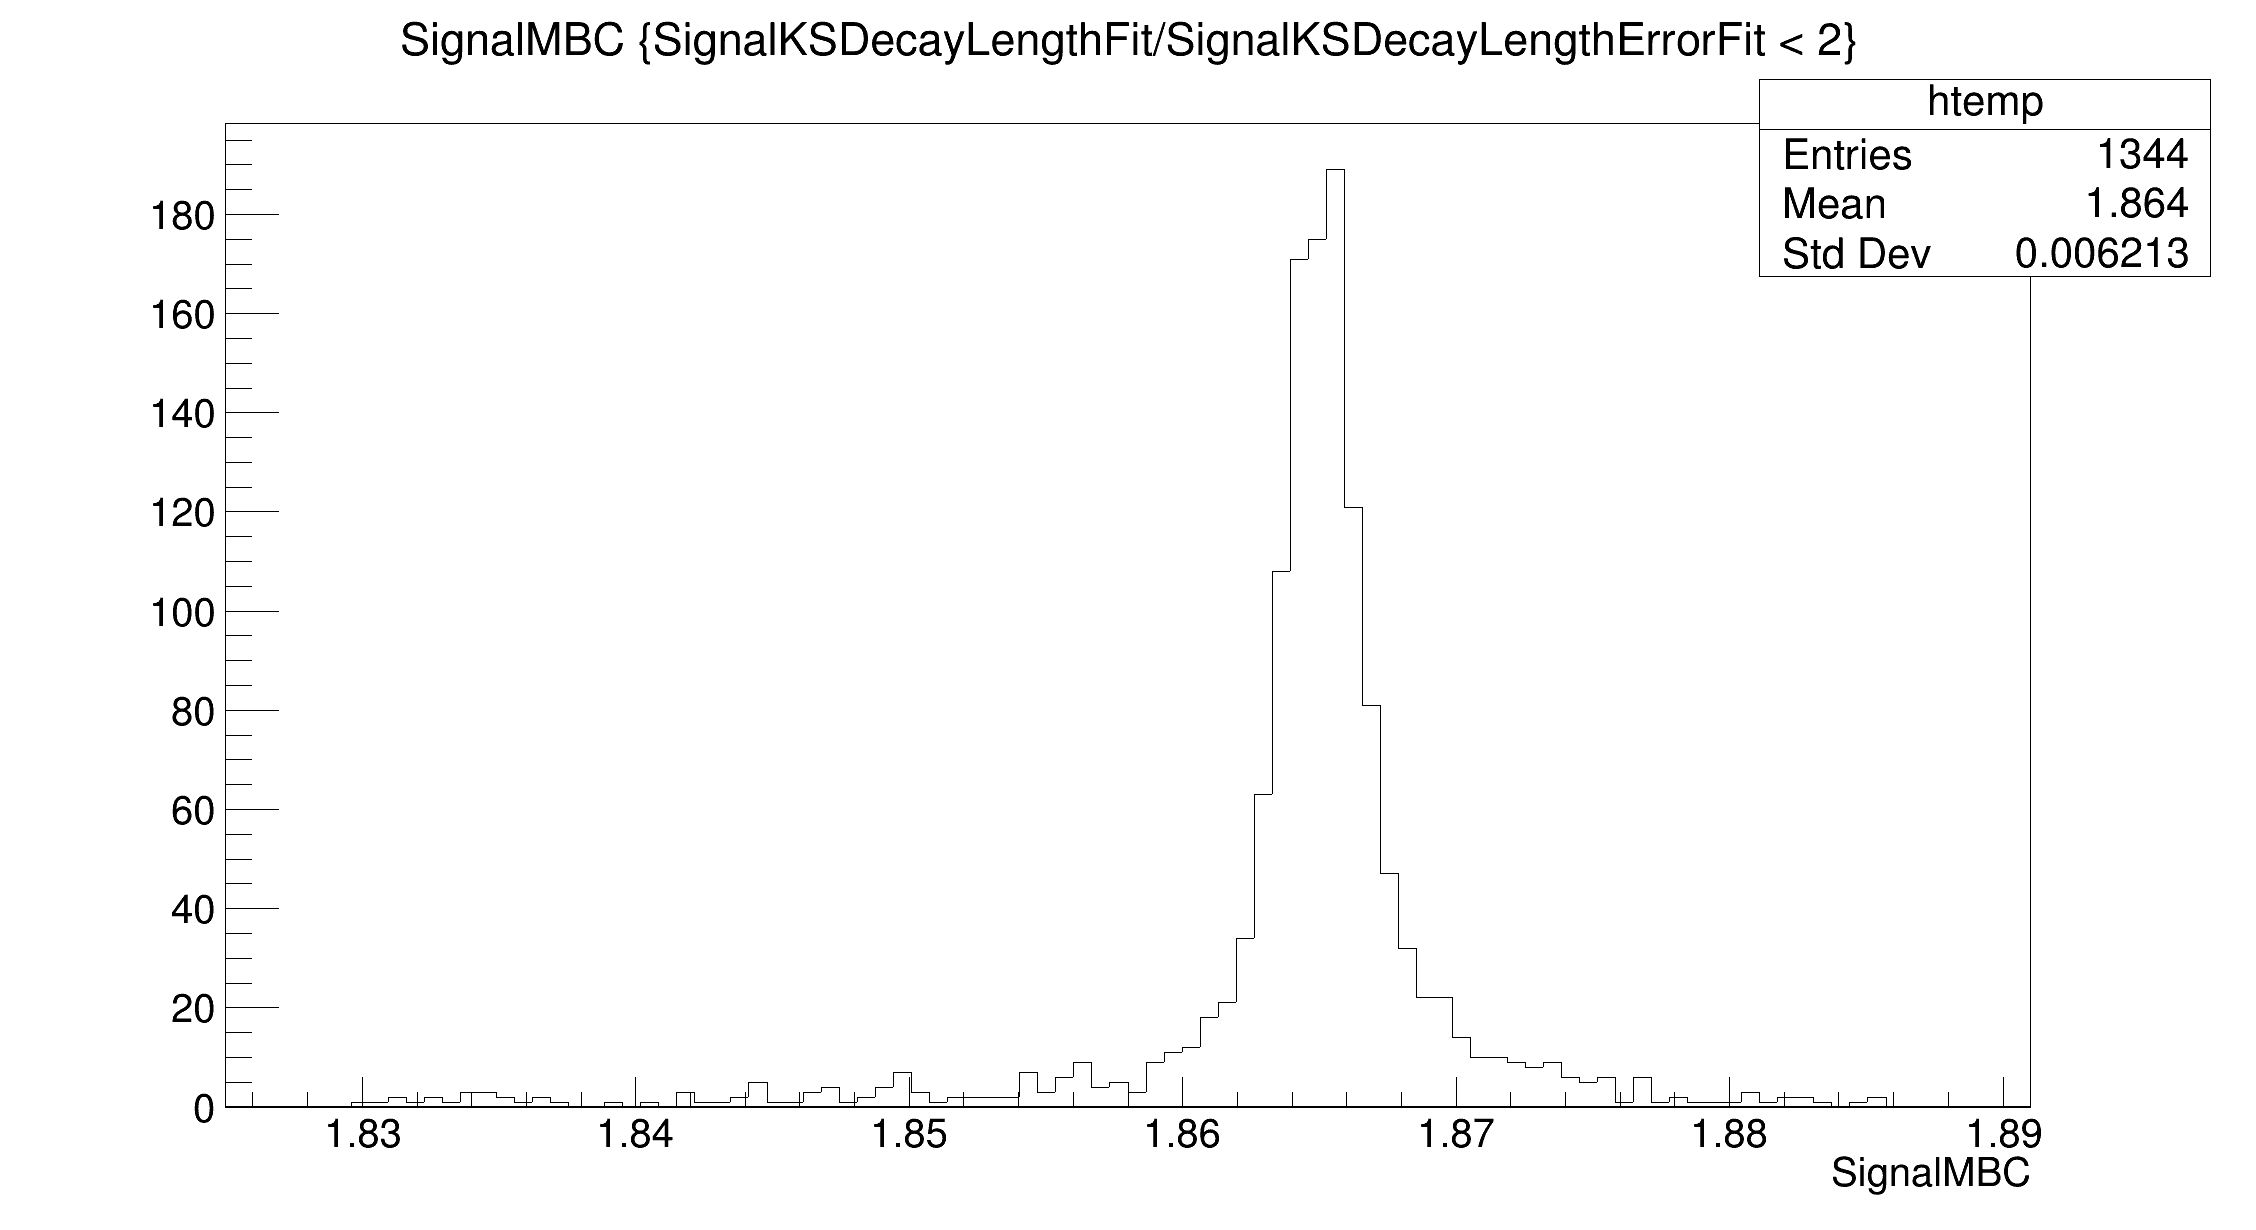
\includegraphics[width=\textwidth]{KpiDoubleTag_SignalMBC.png}
      \caption{$m_{BC}$, $KK\pi\pi$}
    \end{subfigure}%
    \begin{subfigure}{0.5\textwidth}
      \centering
      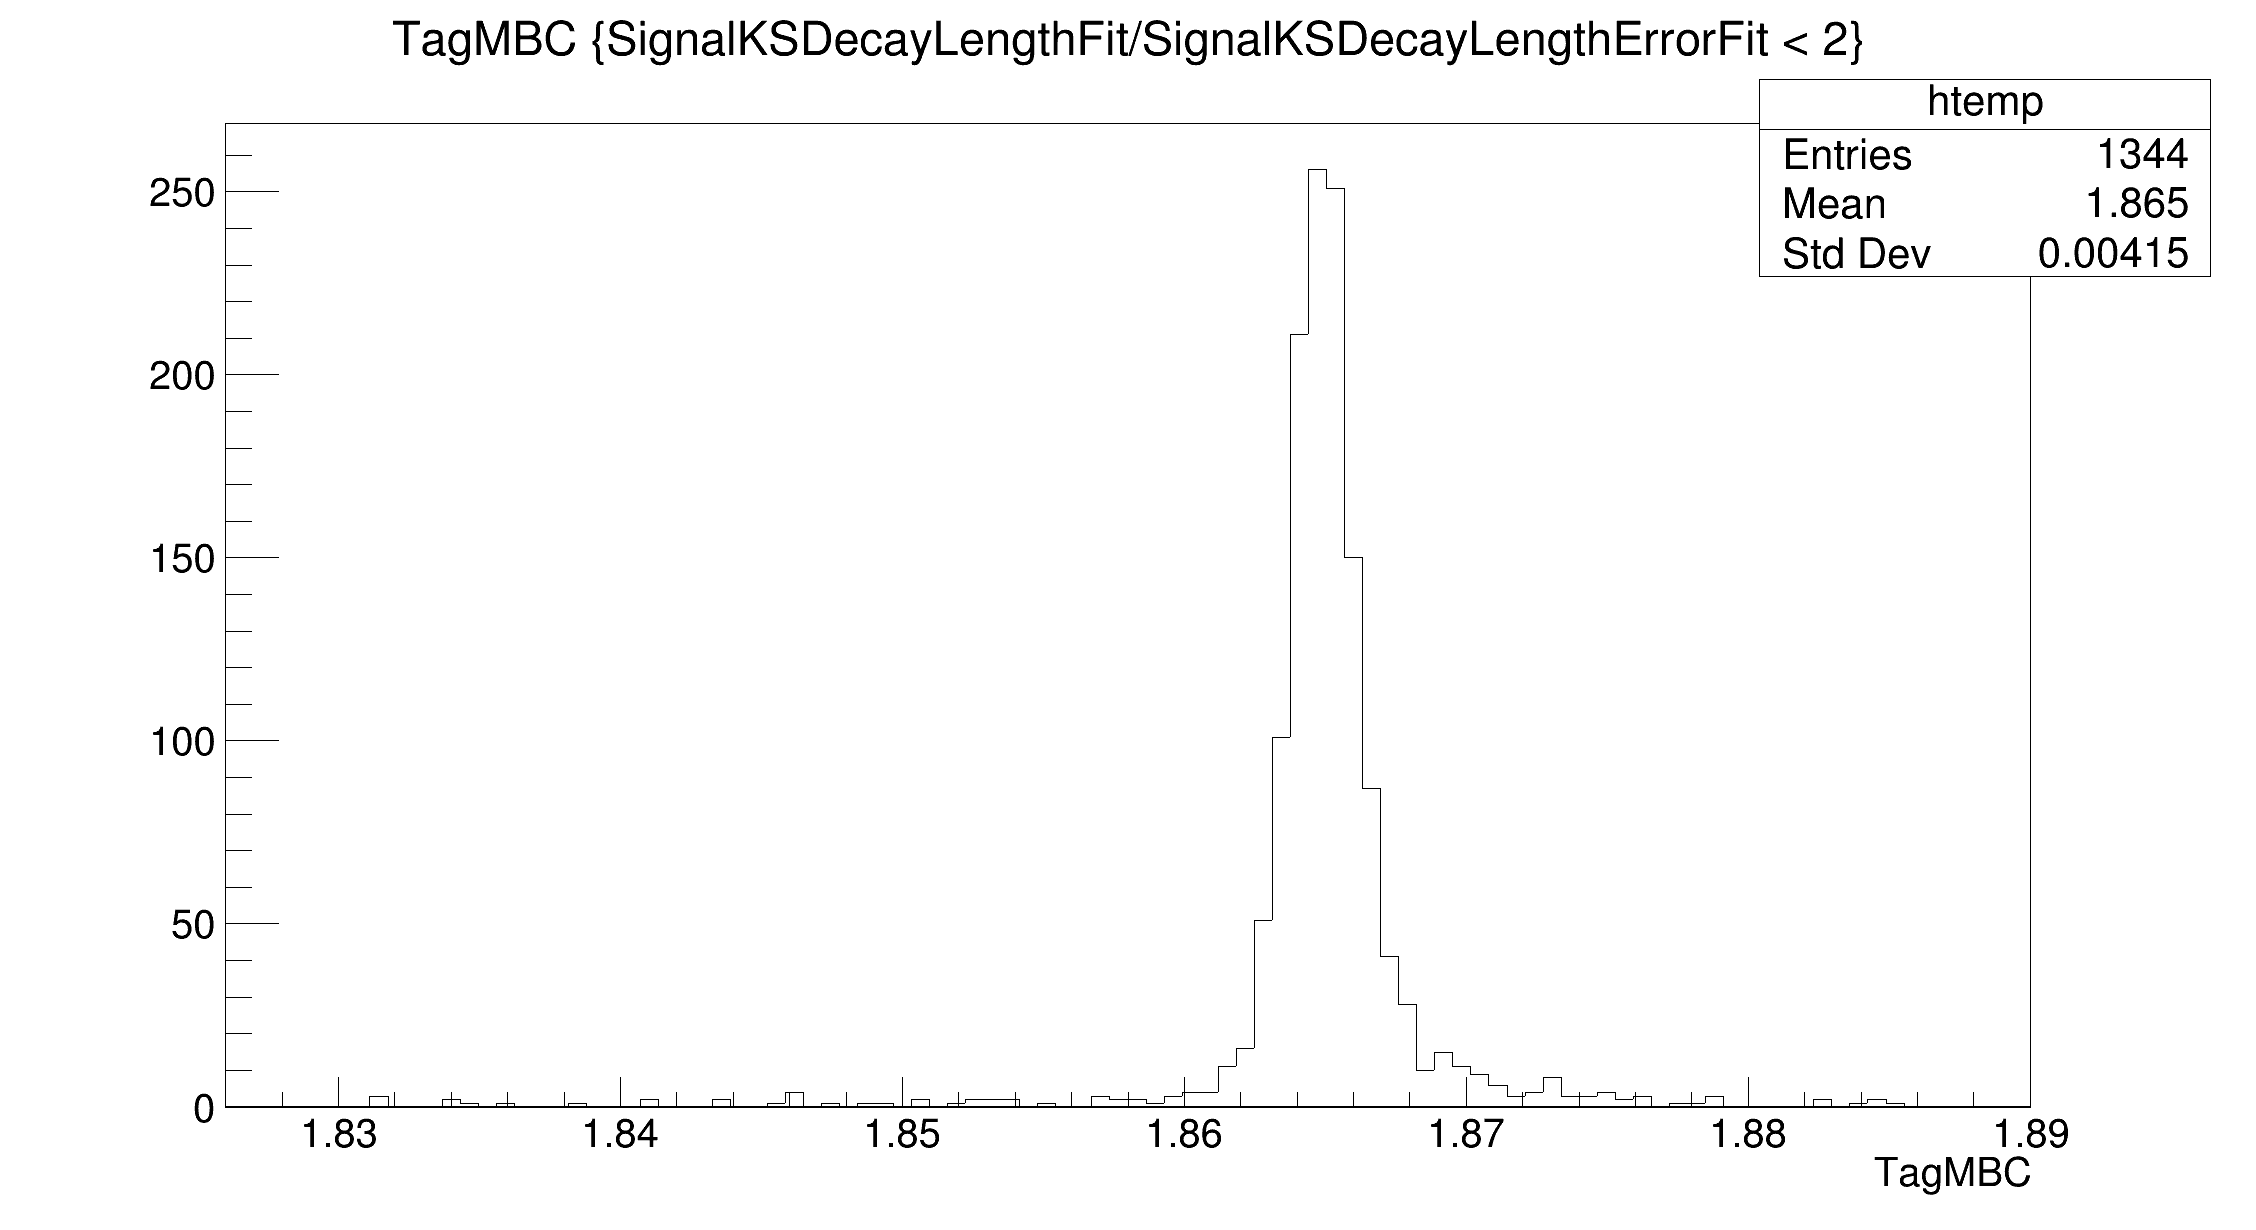
\includegraphics[width=\textwidth]{KpiDoubleTag_TagMBC.png}
      \caption{$m_{BC}$, $K\pi$}
    \end{subfigure}
  \end{figure}
\end{frame}

\begin{frame}{$KK$ tag}
  \begin{figure}
    \centering
    \begin{subfigure}{0.5\textwidth}
      \centering
      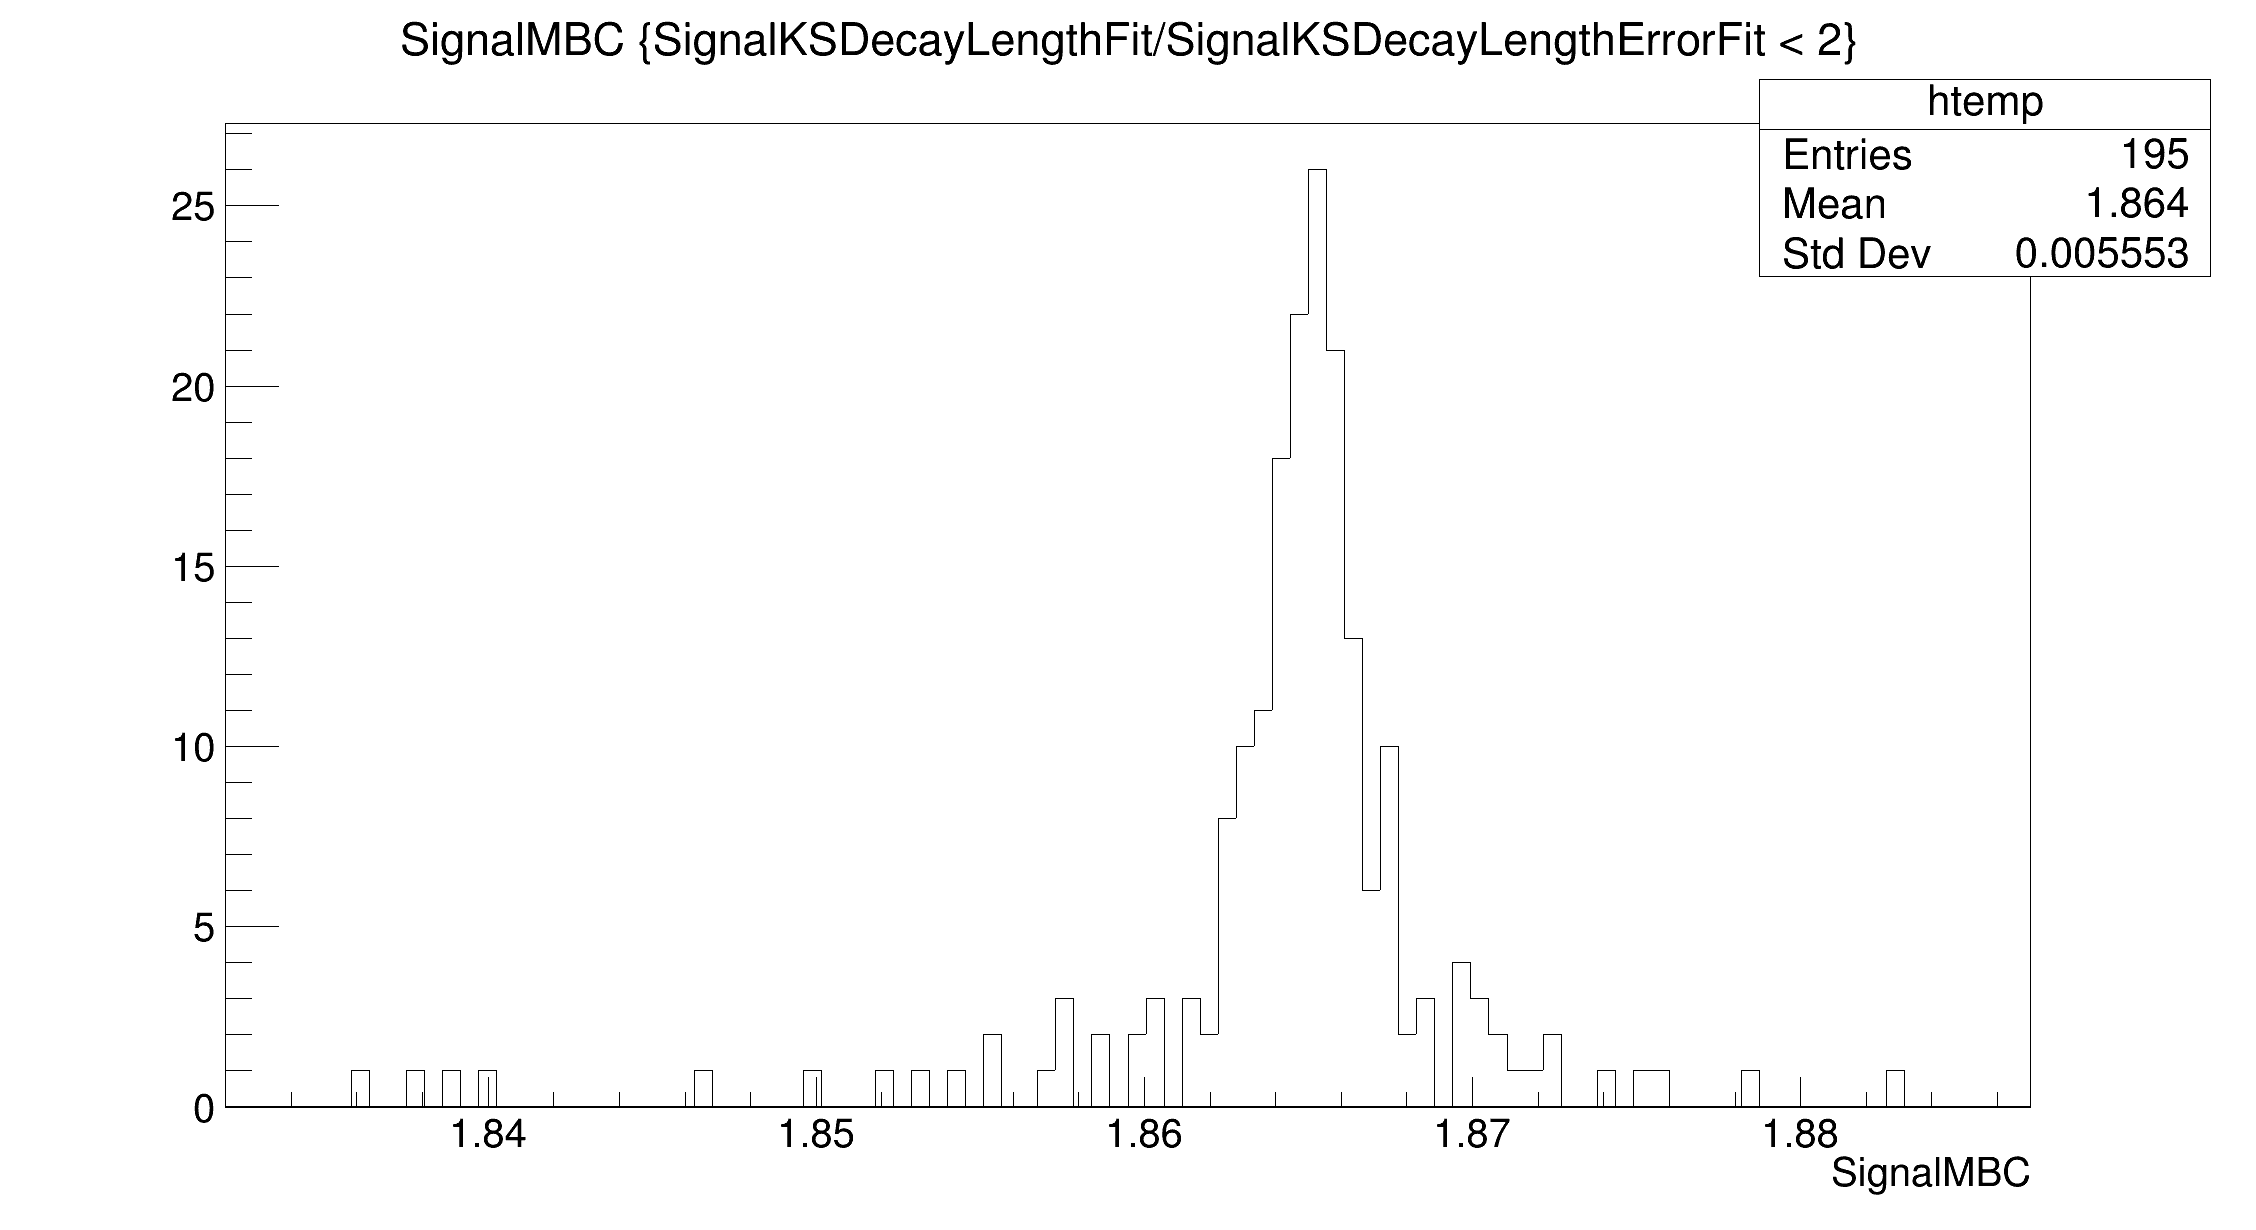
\includegraphics[width=\textwidth]{KKDoubleTag_SignalMBC.png}
      \caption{$m_{BC}$, $KK\pi\pi$}
    \end{subfigure}%
    \begin{subfigure}{0.5\textwidth}
      \centering
      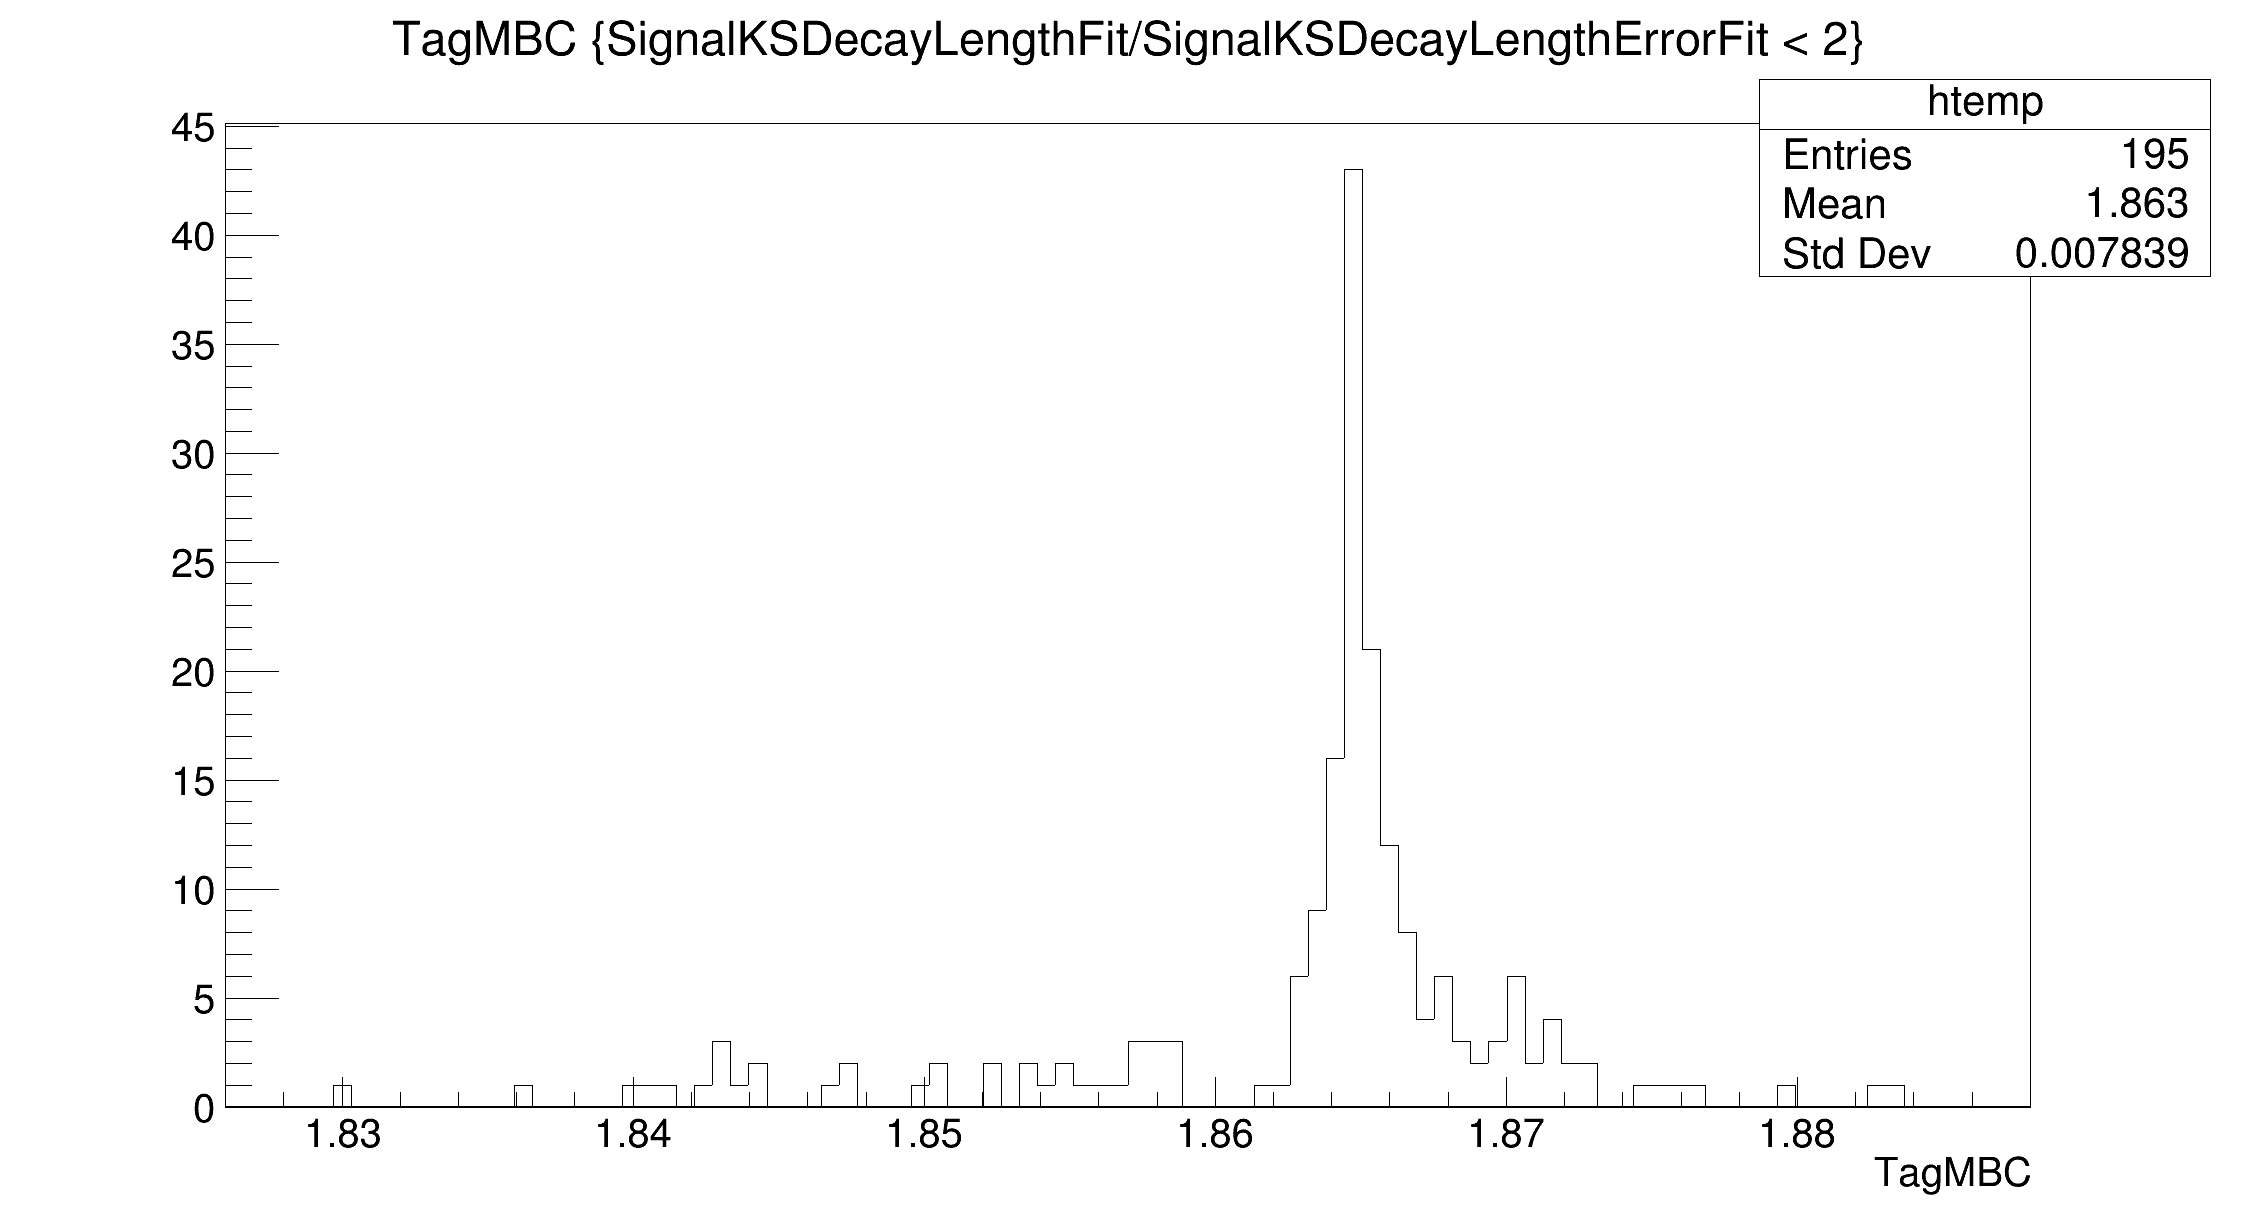
\includegraphics[width=\textwidth]{KKDoubleTag_TagMBC.png}
      \caption{$m_{BC}$, $KK$}
    \end{subfigure}
  \end{figure}
\end{frame}

\begin{frame}{$K_S\pi^0$ tag}
  \begin{figure}
    \centering
    \begin{subfigure}{0.5\textwidth}
      \centering
      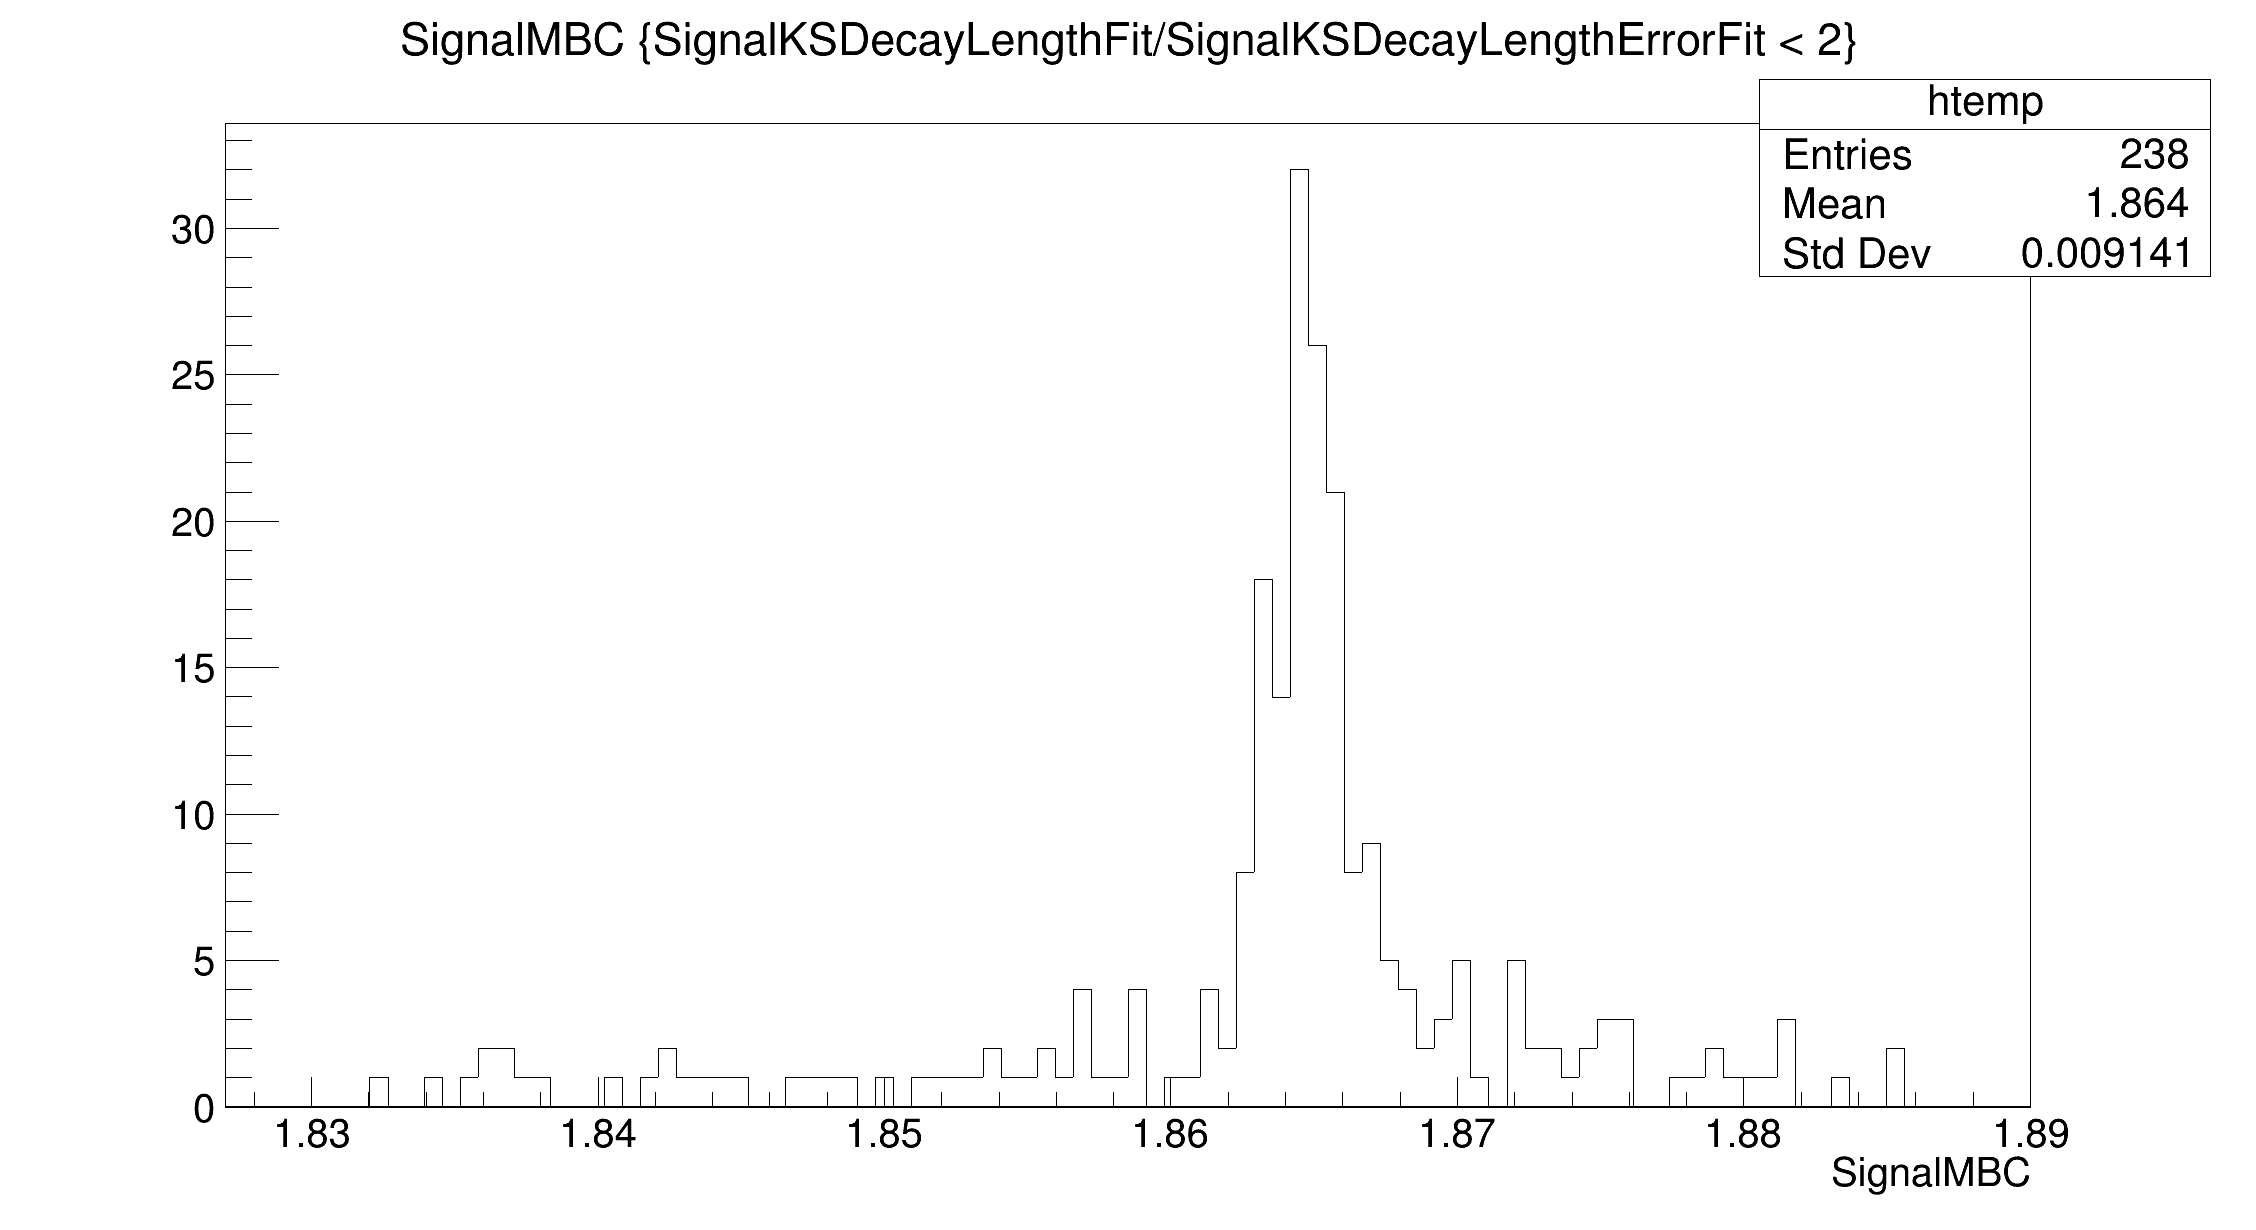
\includegraphics[width=\textwidth]{KSpi0DoubleTag_SignalMBC.png}
      \caption{$m_{BC}$, $KK\pi\pi$}
    \end{subfigure}%
    \begin{subfigure}{0.5\textwidth}
      \centering
      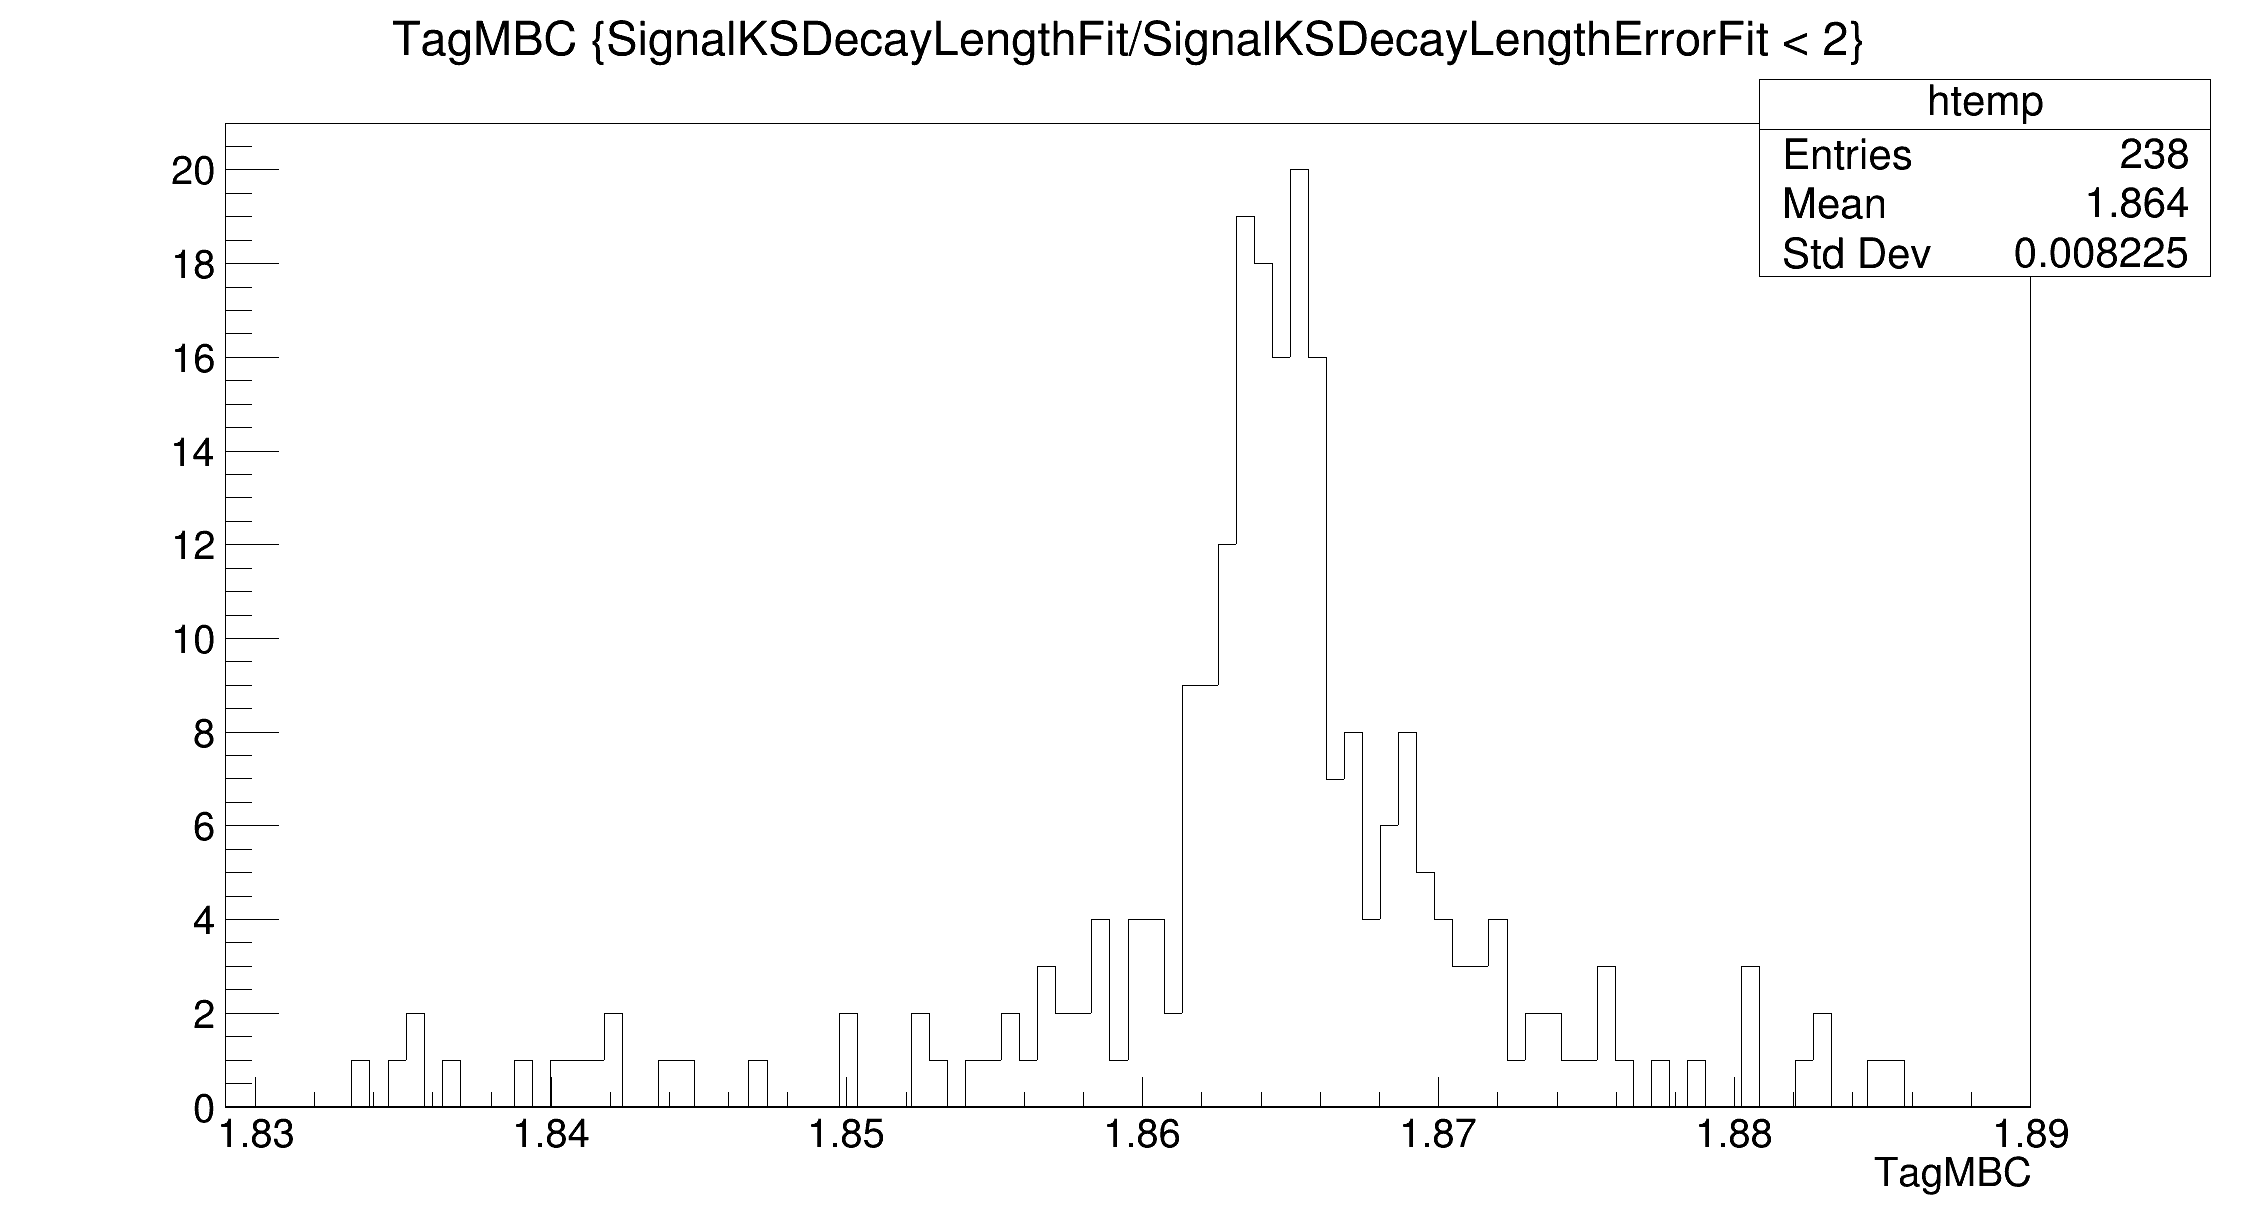
\includegraphics[width=\textwidth]{KSpi0DoubleTag_TagMBC.png}
      \caption{$m_{BC}$, $K_S\pi^0$}
    \end{subfigure}
  \end{figure}
\end{frame}

\begin{frame}{$K\pi\pi^0$ tag}
  \begin{figure}
    \centering
    \begin{subfigure}{0.5\textwidth}
      \centering
      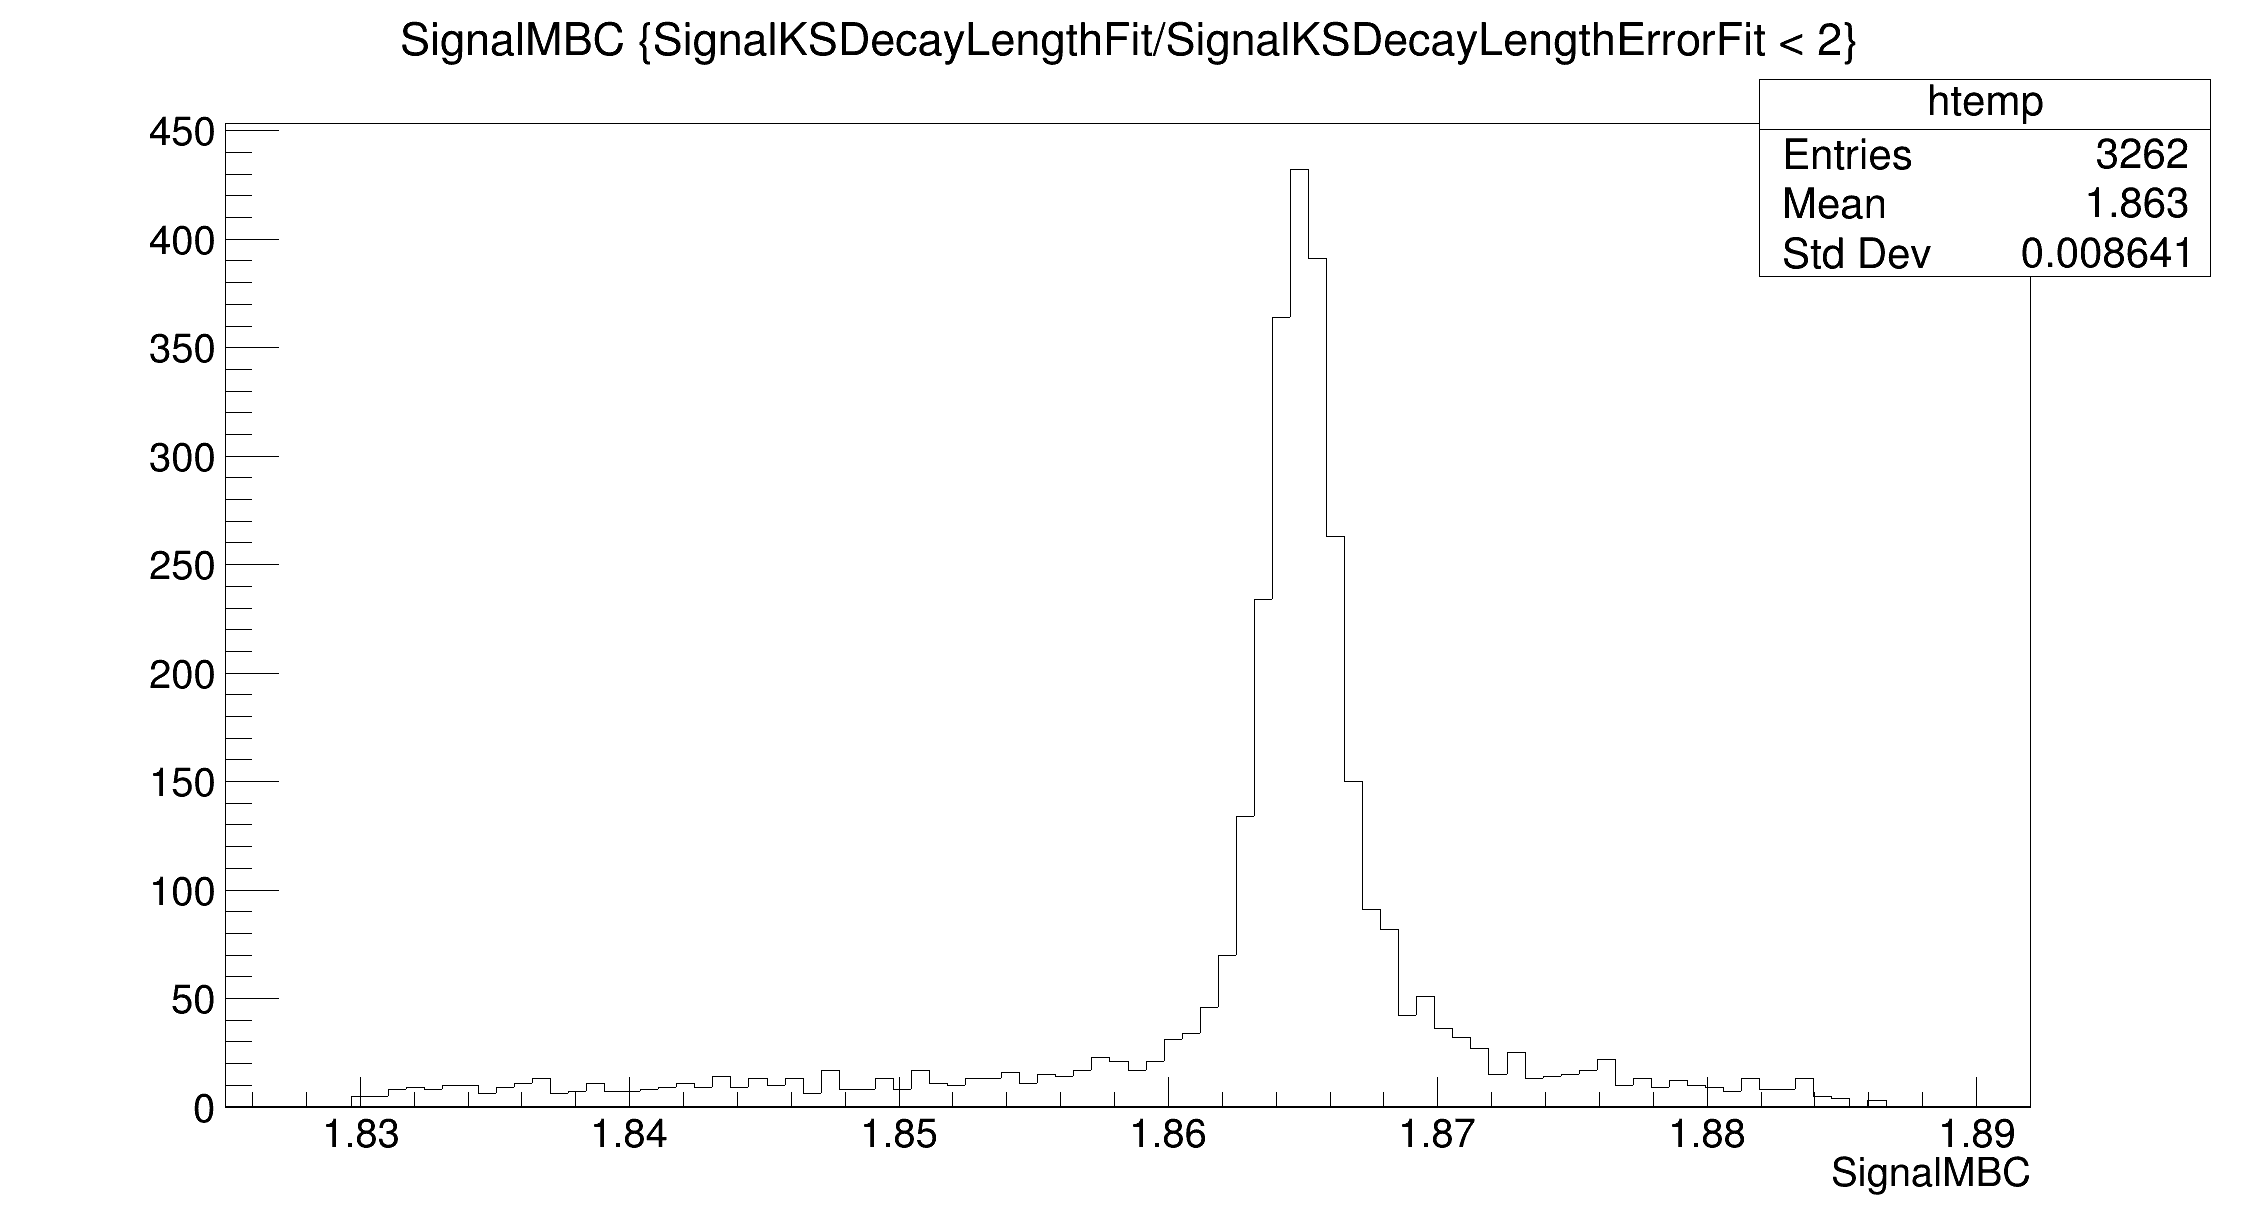
\includegraphics[width=\textwidth]{Kpipi0DoubleTag_SignalMBC.png}
      \caption{$m_{BC}$, $KK\pi\pi$}
    \end{subfigure}%
    \begin{subfigure}{0.5\textwidth}
      \centering
      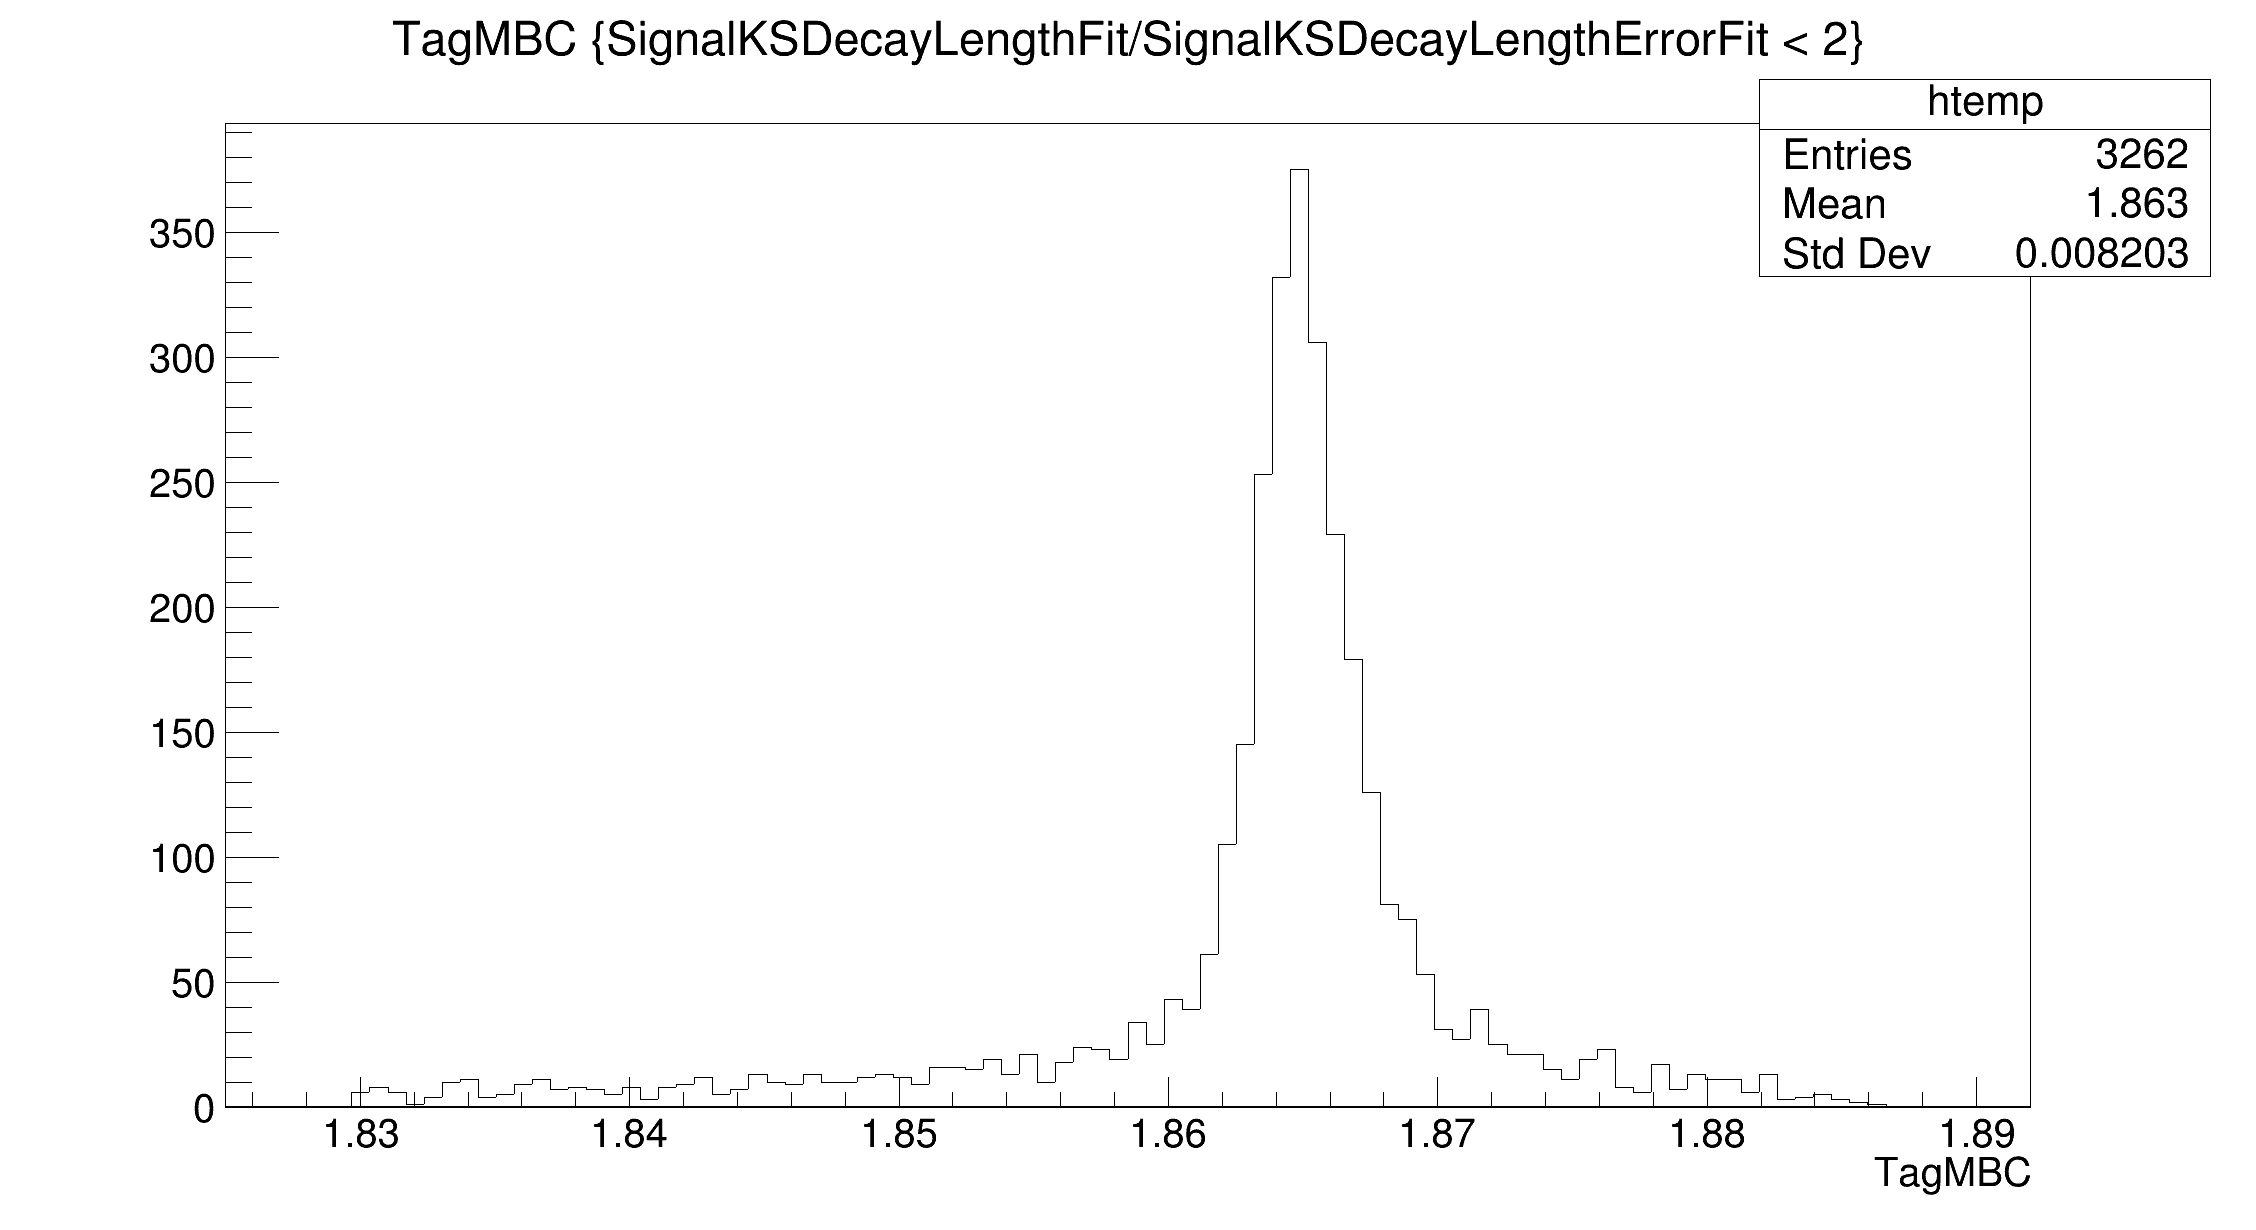
\includegraphics[width=\textwidth]{Kpipi0DoubleTag_TagMBC.png}
      \caption{$m_{BC}$, $K\pi\pi^0$}
    \end{subfigure}
  \end{figure}
\end{frame}

\section{Next steps}
\begin{frame}{Next steps}
  \begin{itemize}
    \item{Include the following modes:}
    \begin{itemize}
      \item{$\pi\pi$, $\pi\pi\pi^0$, $K_S\pi^0\pi^0$, $K_S\eta$, $K_S\omega$}
      \item{$K_L\pi^0$, $K_L\omega$, $K_L\pi^0\pi^0$}
    \end{itemize}
    \item{Run over data}
  \end{itemize}
\end{frame}

\end{document}
